\chapter{Report and discussion of research results}

\section{Part-of-speech tagging}

\subsection{Data}

We extract WSJ articles from the CoNLL-2011 dataset for this experiment. The original data set has already been splitted the into training, development and testing sets so we filter WSJ articles from each set and join the sentences into together. This process results in 11772 sentences for training, 1632 sentences for development and 1382 sentences for testing. The query tested is whether a word has the ``NN'' tag.

We train a HMM model using maximum likelihood principle. For CRF training, we implement the L2-regularized mini-batch AdaGrad method with a batch size of 100.   

\subsection{Results}

\begin{figure}[t]
\minipage{0.32\textwidth}
  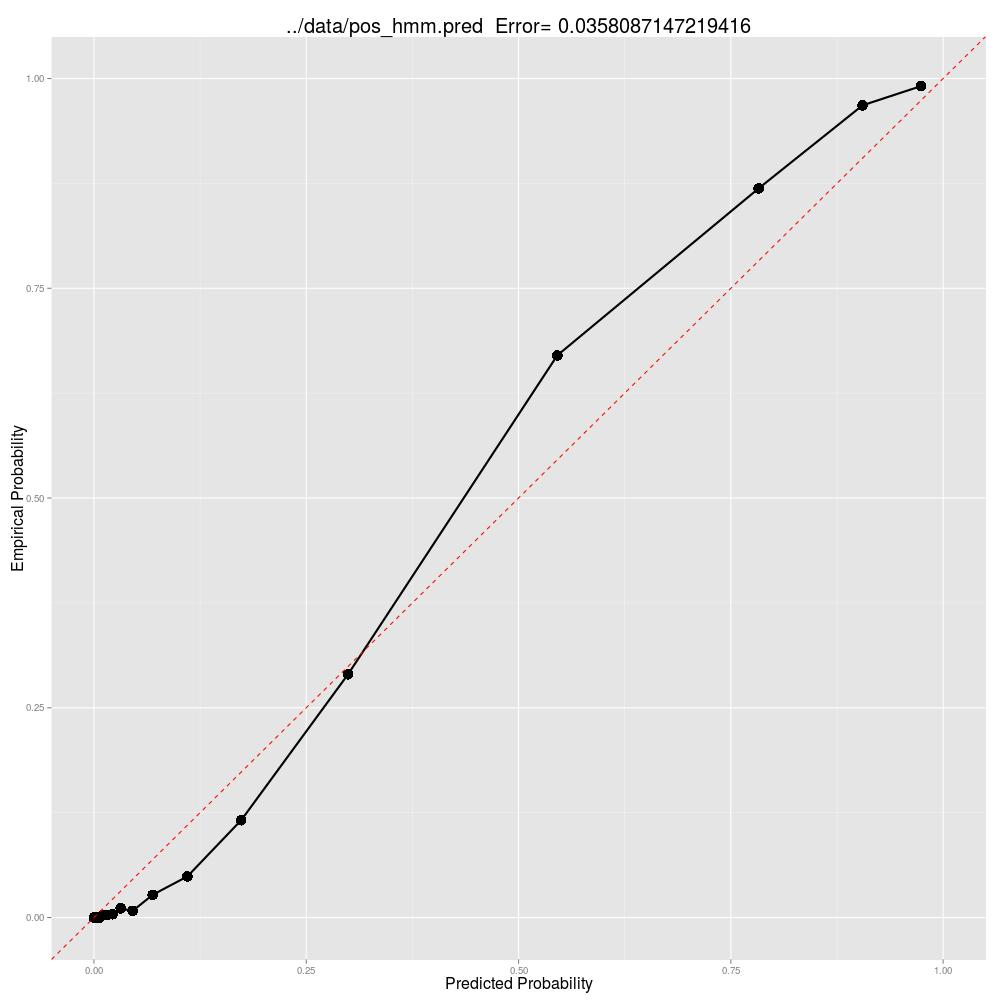
\includegraphics[width=\linewidth, valign=t]{pos_hmm_pred.jpg}
  \caption{Calibration curve for HMM (POS), Acc = ??, CalibScore = ??}
  \label{fig:pos_hmm_pred}
\endminipage\hfill
\minipage{0.32\textwidth}
  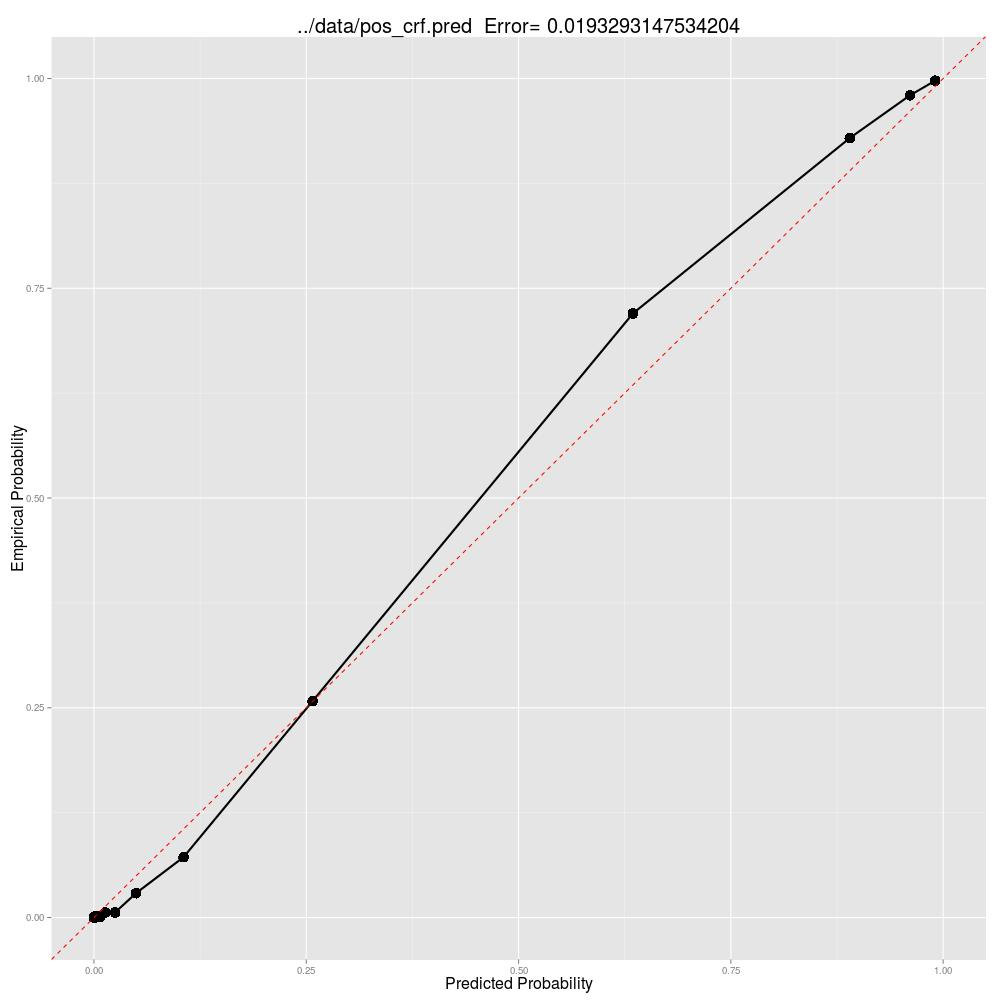
\includegraphics[width=\linewidth, valign=t]{pos_crf_pred.jpg}
  \caption{Calibration curve for CRF-Basic (POS), Acc = ??, CalibScore = ??}
  \label{fig:pos_crf_pred}
\endminipage\hfill
\minipage{0.32\textwidth}
  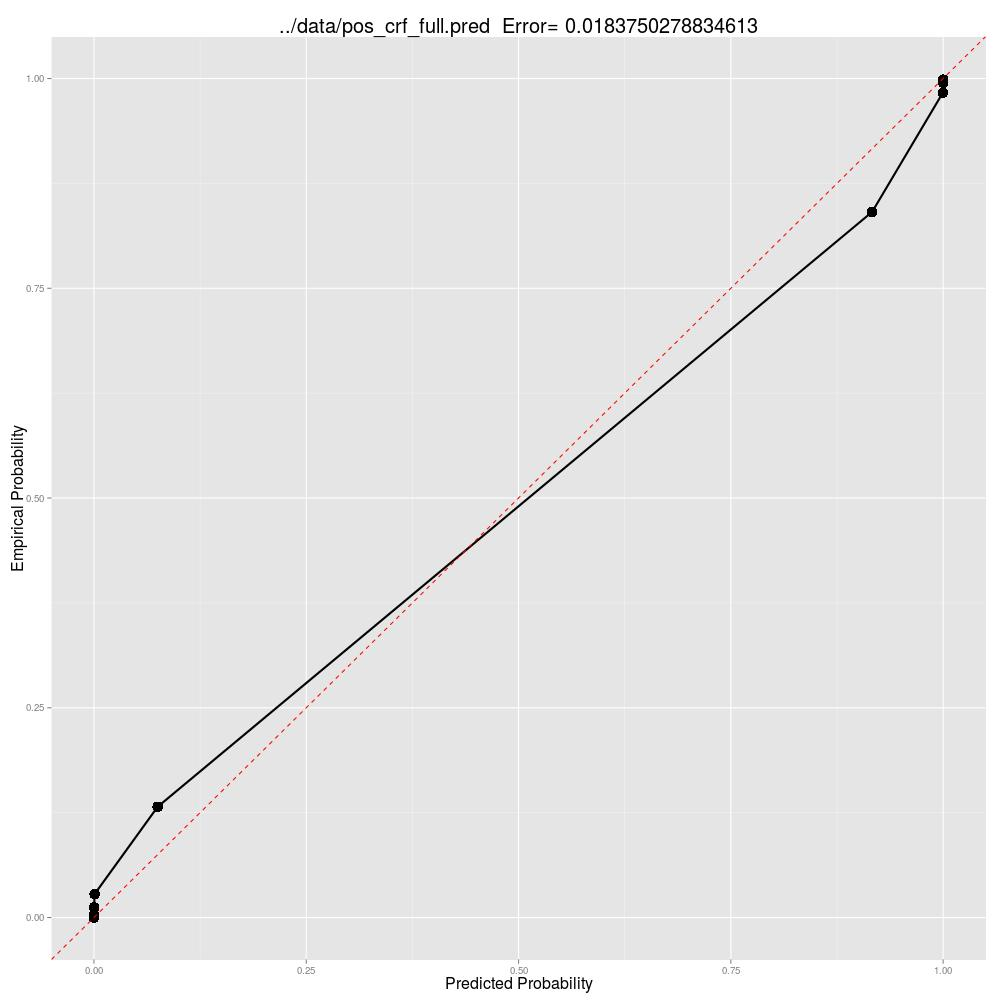
\includegraphics[width=\linewidth, valign=t]{pos_crf_advanced_pred.jpg}
  \caption{Calibration curve for CRF-Advanced (POS), Acc = ??, CalibScore = ??}
  \label{fig:pos_crf_advanced_pred}  
\endminipage
\end{figure}

Firstly, we compare HMM with a CRF model with basic features (CRF-Basic). As mentioned in section 3.4.1, CRF-Basic contains only the transition features and the emission features. Figure \ref{fig:pos_hmm_pred} shows calibration curves of the two models. CRF-Basic attains a significantly lower MSE calibration score than HMM does (0.019 vs. 0.035). Moreover, it also produces more refined predictions than those of HMM, as seen from the distributions of points along the x-axis.

To measure the affect of features on calibration, we conduct an ablation test for CRF. including surrounding words, word shape, word length, prefixes and suffixes. As we discover that as we use better template for CRF, we obtain more refined and calibrated predictions (FIGURE blah blah). A fully featurized CRF, which achieves a 96\% accuraccy on the task, produces a calibration curve just slightly off the PCC. 

\section{Twitter part-of-speech tagging}
\subsection{Data}

We repeat our comparision between HMMs and CRFs on a harder task, predicting POS tags for tweets. We use the ARK's Twitter POS data set (CITE NOAH), which consists of 1000 sentences for training, 327 sentences for development, 500 sentences for testing. The query tested is whether a word has the ``V'' tag. 

We conduct the same experiments as in Section BLAH BLAH and obtain similar patterns. CRF-Basic's miscalibration is about half HMM's (Figure \ref{fig:pos_tweet_hmm_pred}). On the other hand, equipped with better features, CRF-Advanced demonstrates a significant improvement from CRF-Basic, reducing further the miscalibration level by one half. It should also be noticed that CRF-Advanced does not give perfectly accurate predictions (87\% accuracy) but those are reliable predictions.   

\begin{figure}[t]
\minipage{0.32\textwidth}
  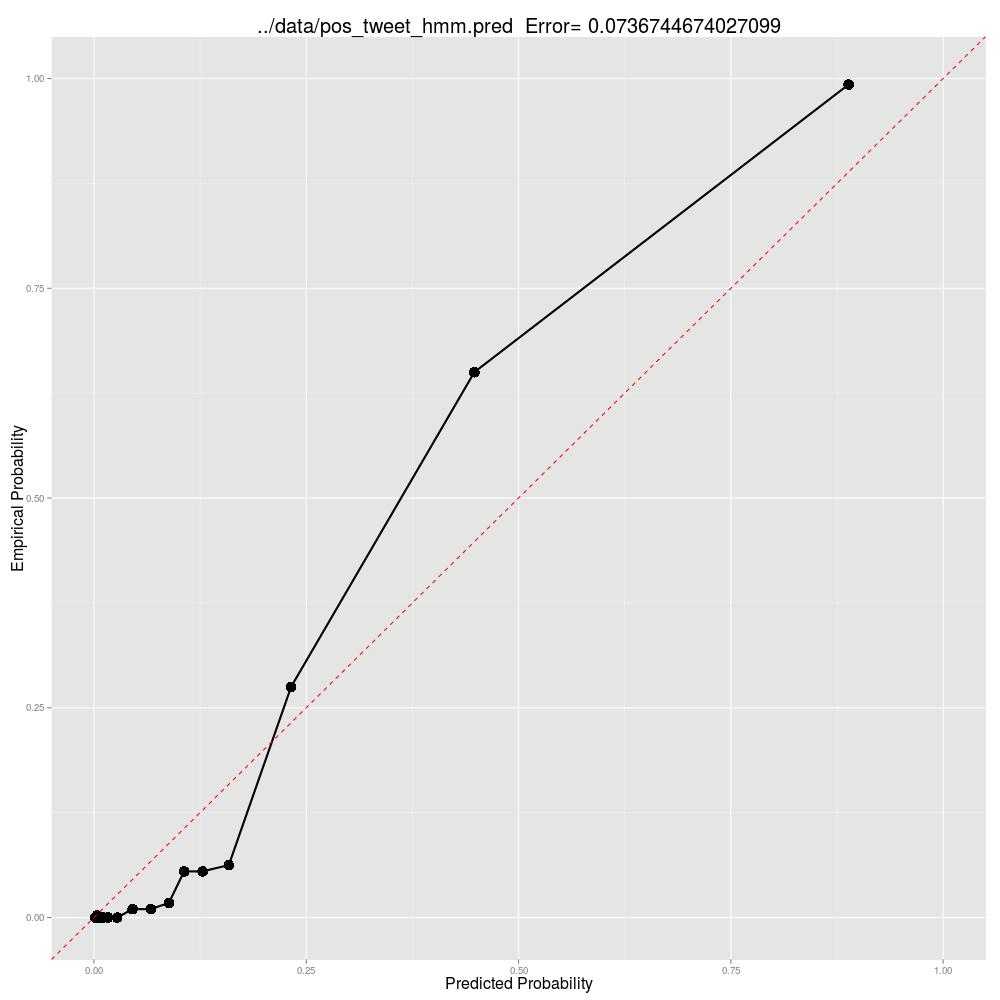
\includegraphics[width=\linewidth]{pos_tweet_hmm_pred.jpg}
  \caption{Calibration curve for HMM (POS Tweet), Acc = ??, CalibScore = ??}
  \label{fig:pos_tweet_hmm_pred}
\endminipage\hfill
\minipage{0.32\textwidth}
  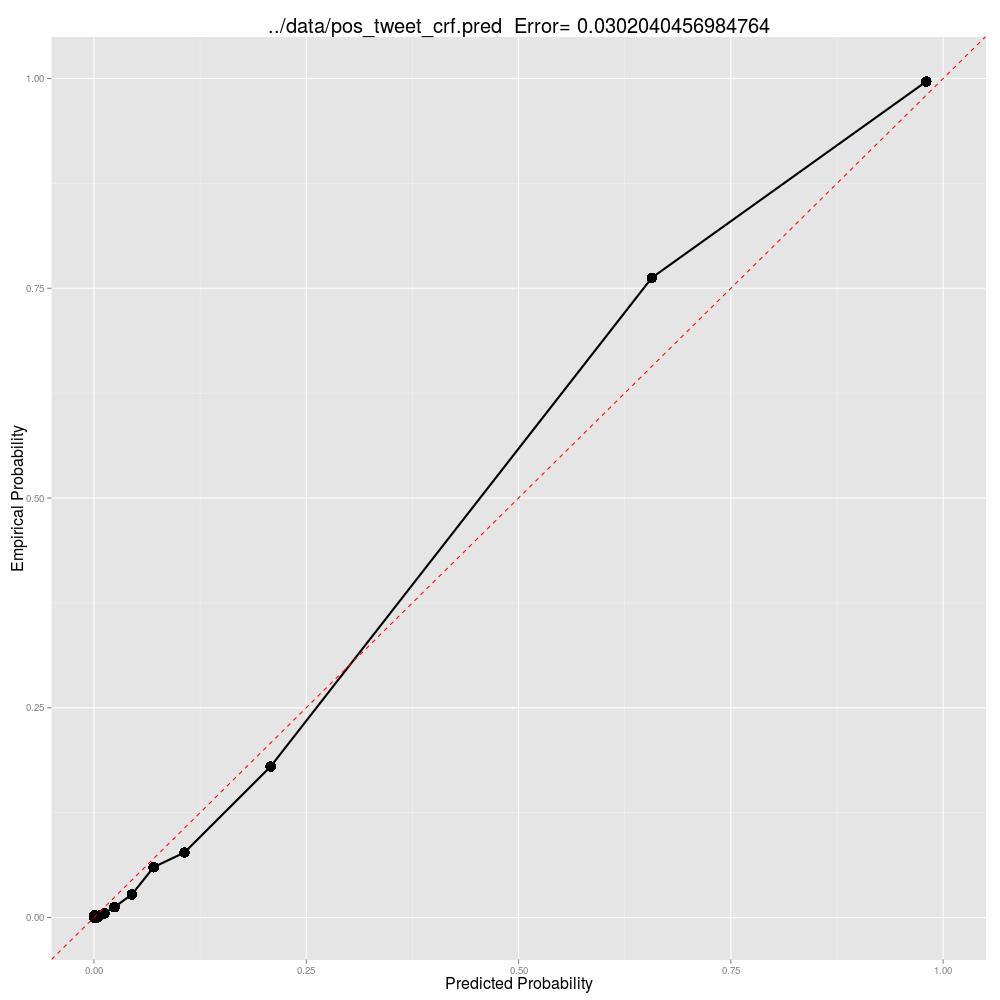
\includegraphics[width=\linewidth]{pos_tweet_crf_pred.jpg}
  \caption{Calibration curve for CRF-Basic (POS Tweet), Acc = ??, CalibScore = ??}
  \label{fig:pos_tweet_crf_pred} 
\endminipage\hfill
\minipage{0.32\textwidth}
  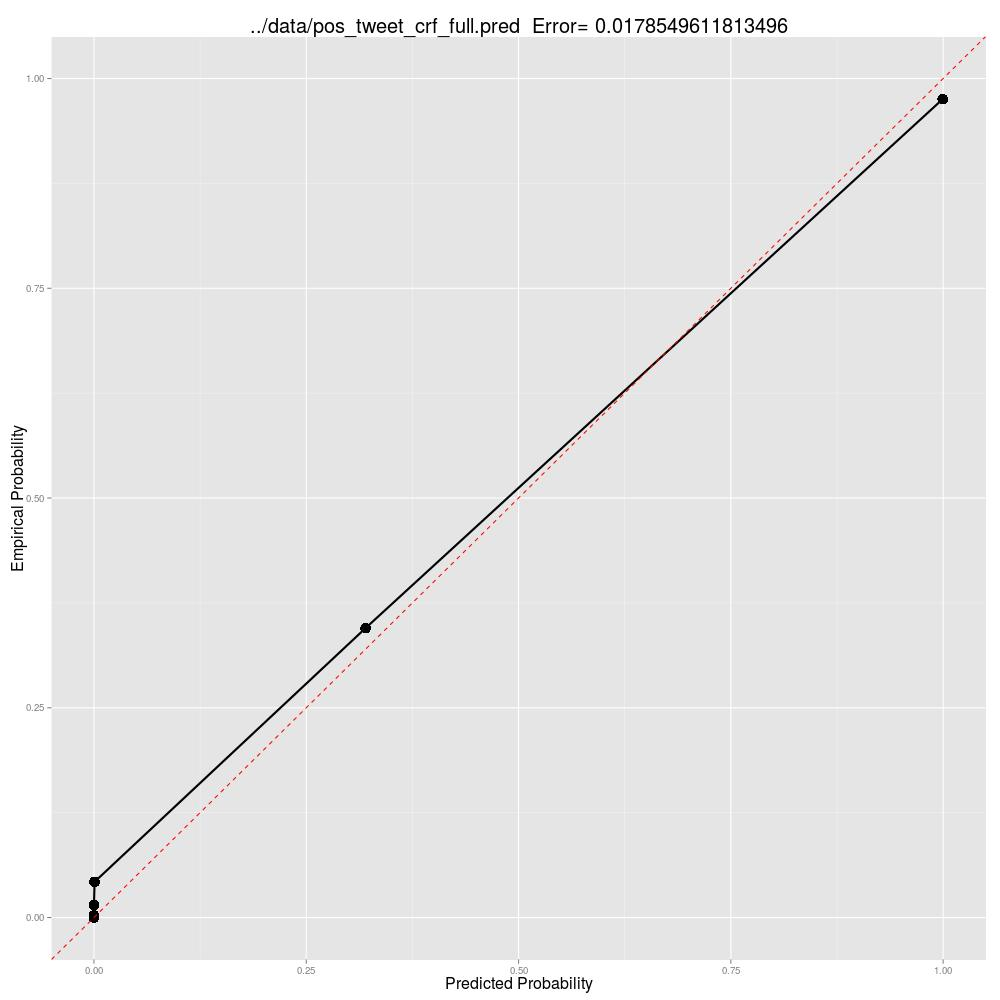
\includegraphics[width=\linewidth]{pos_tweet_crf_advanced_pred.jpg}
  \caption{Calibration curve for CRF-Advanced (POS Tweet), Acc = ??, CalibScore = ??}
  \label{fig:pos_tweet_advanced_crf_pred} 
\endminipage
\end{figure}

